\chapter{Estado da Arte} % (fold)
\label{cap:estado_da_arte}
\acresetall


No estado da arte quanto à representação de topologias de máquina encontra-se o projeto Hardware Locality (hwloc) \cite{hwloc2010}.

O hwloc é um pacote de software amplamente utilizado para a representação de topologias de máquina com grande portabilidade.
Ele contém ferramentas de linha de comando, além de permitir que aplicações acessem as informações sobre a topologia por meio de uma API na linguagem C.



\section{Objetos}
\label{sec:objetos}

Objetos são uma abstração usada para representar todos os elementos presentes na topologia, tanto memória quanto núcleos.
A hierarquia de memória é modelada como uma árvore de objetos, onde cada nível (conjunto de objetos com mesma profundidade) contém objetos de apenas um tipo.
A topologia por completo é representada de forma mais detalhada por meio de várias ligações (ponteiros) entre objetos, conforme as suas relações na hierarquia.
Essas relações são definidas como:
\begin{itemize}
	\item Pai (\textit{parent}): nó pai na estrutura de árvore
	\item Filhos (\textit{children}): nós filhos na estrutura de árvore
	\item Irmãos (\textit{siblings}): nós com o mesmo pai
	\item Primos (\textit{cousins}): Objetos numa mesma profundidade (e, portanto, de mesmo tipo); todos os objetos que compõe um determinado nível (irmãos ou não) são primos
\end{itemize}
% TODO Criar macro
\begin{figure}[h]
	\caption{Relações entre objetos em topologias do hwloc. Fonte: \cite{hwlocImg}}
	\label{fig:relacoes}
	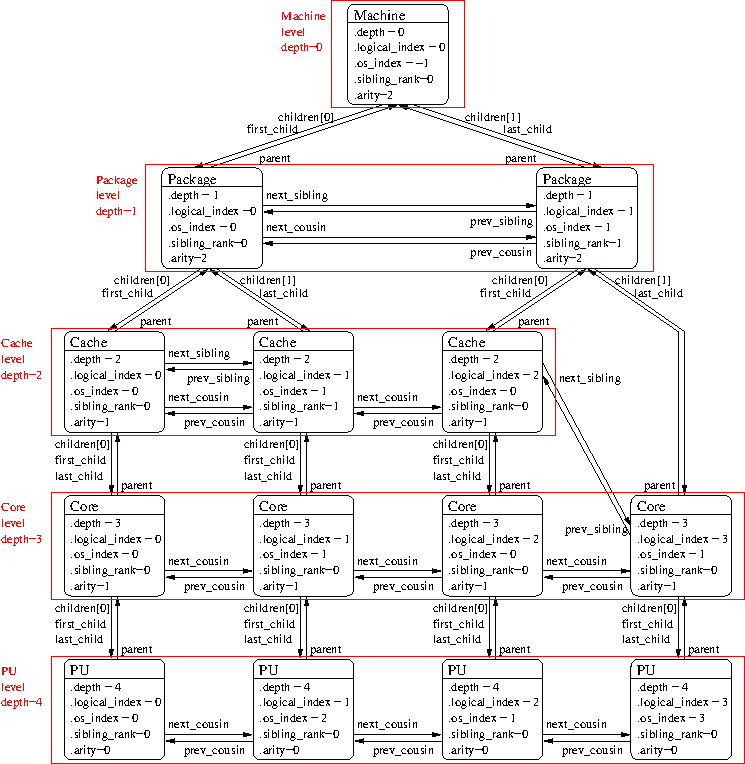
\includegraphics[width=\textwidth]{rec/imagens/relacoes}
\end{figure}
A Figura \ref{fig:relacoes} apresenta um exemplo dessas relações em uma dada topologia.
Ela ilustra, ainda, no ramo mais a direita, o tratamento de assimetrias utilizado pelo hwloc: objetos de um mesmo tipo são emparelhados de modo a compor um mesmo nível.
% [Deixar mais claro] Buracos na hierarquia podem surgir porque o hwloc agrupa objetos do mesmo tipo no mesmo nível.
% Definir assimetria, segundo hwloc. Filhos com graus diferentes resulta em assimetria?
Portanto, objetos irmãos não estarão necessariamente no mesmo nível, e o conceito de profundidade não é exatamente o usado no contexto de estruturas de árvore, sendo possível irmãos terem profundidades diferentes.

Essas relações acrescentadas à estrutura de árvore facilitam a navegação entre objetos, em troca do espaço adicional ocupado por cada ponteiro nos objetos.
Por exemplo, como indicado na figura, a partir de qualquer objeto, é possível navegar para o próximo primo (pelo ponteiro next\_cousin), ou para o próximo irmão (ponteiro next\_sibling), se existirem.
Além disso, todos os objetos são armazenados numa estrutura de array de arrays de objetos, semelhante a uma matriz, mas com arrays internos de tamanho variável.
Cada um dos arrays internos contém os objetos de um nível, e eles são organizados no array externo na ordem dos níveis, de modo que é possível acessar o enésimo objeto de um dado nível diretamente usando essa estrutura.

%Figura X: https://www.open-mpi.org/projects/hwloc/doc/v1.11.2/diagram.png

% >> Conjuntos de CPUs (cpusets)
\section{Conjuntos de CPUs}
\label{sec:conjuntos_de_cpus}

Cada objeto pode ter um cpuset (conjunto de CPUs), que é um mapeamento dos núcleos existentes para bits (bitmap), usado para determinar quais núcleos estão sob o objeto na hierarquia, implementado como uma sequência de variáveis de 32 bits, tantas quantas forem necessárias.
A implementação dos bitmaps poderia ser otimizada para diminuir a quantidade de variáveis utilizadas em casos em que existam grandes quantidades de núcleos.
Algo nesse sentido é citado no respectivo arquivo fonte em um comentário sobre otimizações que poderiam ser realizadas \cite{hwlocCod}.